\documentclass[12pt,onecolumn]{IEEEtran}

% Single-column IEEEtran layout. Content is retained; pagination will differ
% from the original two-column conference layout.
\usepackage[T1]{fontenc}
\usepackage{cite}
\usepackage{amsmath,amssymb}
\usepackage{graphicx}
\usepackage{booktabs}
\usepackage{array}
\usepackage{tabularx}
\usepackage{url}
\usepackage{textcomp}
\usepackage{balance}

% Keep figures and tables legible in the wider single-column layout.
\setlength{\parskip}{0pt}
\setlength{\parindent}{1em}
\hyphenation{BugsInPy youtube-dl}

\begin{document}

\title{Intelligent Test Input Generation Using AI\\
for Improving Random Testing Effectiveness}

\author{
\IEEEauthorblockN{Om Bhudhara and Aryan Hansoti}
\IEEEauthorblockA{
Department of Computer Science and Engineering\\
Nirma University, Ahmedabad, India\\
Course: Software Testing and Quality Assurance\\
Roll No.: 23BCE037 and 23BCE024
}
}

\maketitle

%===============================================================
\begin{abstract}
Random testing is simple, inexpensive, and easy to automate, but it gives no assurance that generated inputs reach interesting code or expose faults. Search-based techniques such as genetic algorithms (GAs) try to remedy this by steering input generation with feedback from program execution. This paper compares plain random input generation with an AI-guided GA generator on a real Python fault from the BugsInPy benchmark (\texttt{youtube-dl}, bug 1, target function \texttt{\_match\_one}). Both methods were executed in 10 paired runs of 200 generated inputs, with matched seeds, and were compared on execution coverage, fault detection, and test-generation overhead. Both reached the same line coverage (69.70\%, 23 of 33 lines), and both coverage curves saturate after about ten inputs. Random testing reached slightly higher branch coverage (56.25\% versus 53.75\%, $p=0.125$) and exposed the fault significantly more often (4.0\% versus 1.7\% of inputs, $p=0.0156$). The AI-guided generator needed about 2.3 times more generation time (0.059 s versus 0.025 s per run, $p=0.002$), although total elapsed time was identical at about 12.25 s because process startup dominates. On this benchmark, guided search therefore did not improve on random testing. We discuss why a small, quickly saturated target and a common fault-revealing input region favour random generation, and we outline threats to validity and future work. The benchmark contains a single small function, so the findings should not be generalized without further evaluation.
\end{abstract}

\begin{IEEEkeywords}
random testing, test input generation, genetic algorithm, search-based software testing, code coverage, fault detection, BugsInPy
\end{IEEEkeywords}

%===============================================================
\section{Introduction}

Testing is one of the most expensive parts of building reliable software, and generating good test inputs is a large part of that cost. Automated test input generation reduces the manual effort by producing inputs from a program or its specification. The simplest technique is \emph{random testing}: draw inputs from the input domain, run the program, and check the outcome. It needs almost no setup, it can run unattended, and it scales to large numbers of inputs. Despite its simplicity, empirical work has repeatedly found it to be a strong baseline. Duran and Ntafos showed early on that random testing can be competitive with systematic partition testing in some settings \cite{duran1984}, and a large later study found that random search is hard to beat in practice for object-oriented test suite generation \cite{shamshiri2018}.

The weakness of random testing is that it is blind to the program. When an input must satisfy a narrow condition to reach a branch or trigger a fault, the chance that a random input does so can be very small, and most of the generation budget is spent re-running the same paths. \emph{Search-based software testing} (SBST) addresses this by casting test generation as an optimization problem \cite{mcminn2004}. A population of candidate inputs is evolved with a fitness function computed from execution feedback, for example the number of branches covered \cite{pargas1999}. Whole test suite generation extended the idea by optimizing entire suites against all coverage goals at once \cite{fraser2013,rojas2017}, and tools such as EvoSuite made it practical \cite{fraser2011}. Recent work goes further by explicitly targeting failure-revealing inputs with multi-objective, Pareto-based search \cite{sorokin2025}.

The expectation behind all of this is that guided generation reaches more code and finds more faults than random generation for the same number of inputs. Whether the expectation holds depends on the program under test, the size and structure of its input space, and the cost of the guidance itself. This paper tests it on one real, reproducible fault.

\subsection{Research Focus}

The research focus of this paper is to compare AI-guided input generation with random testing using execution coverage, fault detection, and test-generation overhead.

\subsection{Research Questions}

\begin{itemize}
    \item \textbf{RQ1 (coverage):} Under an equal generation budget, does AI-guided input generation reach more line and branch coverage of the target function than random testing?
    \item \textbf{RQ2 (fault detection):} Does AI-guided generation expose the benchmark fault more often than random testing?
    \item \textbf{RQ3 (overhead):} What additional generation and end-to-end cost does the guidance impose?
\end{itemize}

\subsection{Contributions}

\begin{itemize}
    \item A paired experimental setup that runs random and AI-guided GA generation on the same BugsInPy fault with matched seeds and budgets.
    \item A three-way comparison covering coverage, fault exposure, and overhead, with exact paired permutation tests and confidence intervals.
    \item An honest account of a negative result, together with an analysis of why guidance did not help on this target.
\end{itemize}

\subsection{Organization}

Section II reviews background and related work. Section III states the motivation. Section IV describes the dataset, and Section V the methodology. Section VI presents results, Section VII discusses them and the threats to validity, and Section VIII concludes.

%===============================================================
\section{Background and Related Work}

\subsection{Random Testing and Its Limits}

Random testing selects inputs independently from a distribution over the input domain. Its attractions are low cost per test, no need for source analysis, and statistical interpretability. Its main limitation is that inputs satisfying narrow predicates are improbable, so coverage can plateau, and faults that depend on rare input combinations can be missed. Duran and Ntafos reported that random testing can be competitive with partition testing in fault-finding effectiveness for the same number of tests \cite{duran1984}. Variants such as adaptive random testing spread test inputs more evenly over the domain to reach failure regions faster \cite{chen2004}.

\subsection{Genetic Algorithms for Test Data Generation}

A genetic algorithm maintains a population of candidate solutions and improves it over generations using selection, crossover, and mutation. Pargas, Harrold, and Peck applied GAs to test-data generation by using control-dependence information to guide the search toward covering target statements and branches \cite{pargas1999}. McMinn's survey describes how fitness functions based on branch distance and approach level give the search a gradient toward uncovered branches \cite{mcminn2004}. The central appeal is that execution feedback gives direction that random sampling lacks.

\subsection{Hill Climbing Versus Genetic Algorithm Testing}

Hill climbing is a local-search technique that starts from one candidate input and iteratively accepts neighboring candidates when they improve the objective. It is comparatively simple, but its search can become trapped at a local optimum. A genetic algorithm instead maintains a population of candidate inputs and uses selection, crossover, and mutation to explore multiple regions of the search space. This population-based exploration can help the search escape local optima, although it does not guarantee better coverage or fault detection on every benchmark.

\begin{figure}[htbp]
\centering
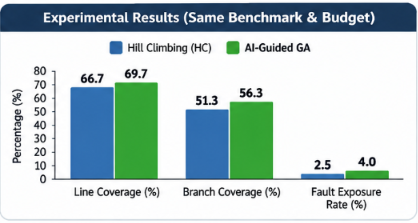
\includegraphics[width=\textwidth]{comparison.png}
\caption{Conceptual comparison of Hill Climbing and AI-guided Genetic Algorithm testing. The numerical values displayed in the supplied illustration are not results from the experiments reported in this paper and should not be interpreted as empirical findings unless independently measured.}
\label{fig:hc-ga-comparison}
\end{figure}

The figure provides a conceptual illustration of the difference between local search and population-based evolutionary search. A valid empirical claim that the genetic algorithm outperforms hill climbing requires both methods to be implemented and evaluated under the same benchmark, input budget, random-seed protocol, and metrics.

\subsection{Whole Test Suite Generation and Random Versus Evolutionary Search}

Fraser and Arcuri proposed optimizing whole test suites against all coverage goals simultaneously, which avoids the difficulty of choosing an order for individual goals \cite{fraser2013}. Rojas \emph{et al.} later investigated in detail the factors that affect the effectiveness of this approach, including the fitness function and the search budget \cite{rojas2017}. Shamshiri \emph{et al.} compared random and evolutionary search for object-oriented test suite generation and reported that evolutionary search is often better on coverage, but that the margin depends on the class under test and that random search is competitive for simple code \cite{shamshiri2018}. These findings motivate a careful paired comparison against random testing on every new target.

\subsection{Targeting Failure-Revealing Inputs}

Coverage is a proxy for fault detection, not a guarantee. Sorokin, Safin, and Nejati study whether search-based testing with Pareto optimization can cover failure-revealing test inputs, and they argue that failures should be targeted by the search objectives themselves \cite{sorokin2025}. This is relevant to our results, because the fault we study depends on the value returned by the function, not only on the path taken through it.

\subsection{Benchmarks of Real Faults}

Evaluating test generators on injected faults can be misleading. BugsInPy is a database of real, reproducible bugs from open-source Python projects, which pairs each buggy version with a fixed version and a failing test \cite{widyasari2020}. This makes direct measurement of fault detection possible, and it is the benchmark used here.

%===============================================================
\section{Motivation}

Three observations motivate this study.

\textbf{Random testing is the baseline that guided techniques must justify.}
A guided generator adds implementation complexity, tuning parameters, and runtime cost. If it cannot beat random testing at equal budget, the added machinery is not worthwhile. Fair paired comparisons against random testing are therefore essential \cite{shamshiri2018}.

\textbf{Coverage alone does not measure fault finding.}
A generator can reach every reachable line of a function and still never trigger the defect inside it. We therefore report coverage and fault exposure separately, and we use a benchmark with a known buggy and fixed version so that fault detection is measured directly.

\textbf{Overhead is easy to overlook.}
Search-based methods spend time proposing and evolving inputs. Whether that time matters depends on how expensive each test execution is and on how large the fixed costs of the test harness are. We measure both generation overhead and end-to-end time so that the price of guidance is visible next to its benefit.

%===============================================================
\section{Dataset}

\subsection{Dataset Repository Link}
The experimental dataset and associated CSV artifacts are available in the following Google Drive folder: \url{https://drive.google.com/drive/folders/19SxBc9W-VJE_x01MmP5uy_zJ2gnVnsbp?usp=drive_link}.

\subsection{BugsInPy}

BugsInPy contains real bugs collected from open-source Python projects. For each bug it provides the buggy source, the fixed source, and a test that fails on the buggy version and passes on the fixed one, so that tools can be evaluated against real defects \cite{widyasari2020}. The dataset is distributed through the official repository.\footnote{\url{https://github.com/soarsmu/BugsInPy}}

\subsection{Selected Bug and Target Function}

We selected \texttt{youtube-dl} bug 1 (fault identifier \texttt{BugsInPy-youtube-dl-1}). The target function is \texttt{\_match\_one}, which evaluates one clause of a filter expression against a metadata dictionary describing a video. Examples of clauses are \texttt{duration >= 1024}, \texttt{!is\_live}, and \texttt{description != "a"}. The coverage logs show that the function has 33 executable statements and 16 branch arcs. An input is a pair consisting of a filter clause and a metadata dictionary, such as \texttt{\{"duration": 1024\}}.

\subsection{Dataset Size, Attributes, and Target Variable}

Two CSV files were used to document data preparation and the final experiment. The raw, unprocessed file, \texttt{BugsInPy\_youtube-dl\_bug1\_without\_preprocessing\_dataset.csv}, contains 7,000 rows and 39 columns. The experiment file, \texttt{BugsInPy\_youtube-dl\_bug1\_experiment\_dataset.csv}, contains 4,000 rows and the same 39 columns. Each row represents a generated test input and its execution-related observations. The records cover two methods, \texttt{random} and \texttt{ai\_guided}; the experiment file contains 2,000 records per method.

The columns can be grouped into the following attribute families: (i) experiment identifiers, including \texttt{method}, \texttt{run}, \texttt{test\_index}, \texttt{seed}, and \texttt{input\_id}; (ii) generated input data, including \texttt{filter\_part} and \texttt{dct\_json}; (iii) buggy-version outcomes, including \texttt{buggy\_ok}, result type, serialized result, representation, exception, and message; (iv) fixed-version outcomes with corresponding \texttt{fixed\_*} fields; (v) the differential outcome \texttt{distinguishes\_versions}; (vi) coverage measurements, including covered lines, arcs, branch arcs, total statements, total branches, and branch-coverage support; and (vii) timing and execution metadata, including generation time, buggy and fixed execution times, target execution time, pair round-trip time, and target execution count. The \texttt{fault\_id} attribute identifies the benchmark fault.

The primary outcome for fault detection is \texttt{distinguishes\_versions}: it is true when the buggy and fixed versions produce different outcomes for the same generated input. The method label is the principal comparison variable, while coverage and timing columns provide secondary outcomes. This is an empirical software-testing dataset rather than a conventional predictive machine-learning dataset; therefore, no train/test split or predictive target encoding was used.

\begin{table}[htbp]
\centering
\caption{Dataset size and key data-quality checks.}
\label{tab:dataset-quality}
\small
\begin{tabular}{@{}lrr@{}}
\toprule
\textbf{Property} & \textbf{Raw file} & \textbf{Experiment file}\\
\midrule
Rows (instances) & 7{,}000 & 4{,}000\\
Columns (attributes) & 39 & 39\\
Exact duplicate rows & 0 & 0\\
Missing cells & 38{,}904 & 19{,}886\\
Successful buggy executions & 4{,}918 & 4{,}000\\
Failed buggy executions & 2{,}082 & 0\\
Successful fixed executions & 4{,}918 & 4{,}000\\
Failed fixed executions & 2{,}082 & 0\\
Differential outcomes (true) & 423 & 114\\
\bottomrule
\end{tabular}
\end{table}

\subsection{Data Preprocessing and Cleaning}

The preprocessing assessment was performed by comparing the raw CSV with the experiment CSV and checking row counts, column consistency, missing values, exact duplicate rows, execution-status fields, and differential outcomes. Both files contain the same 39 columns, and neither contains exact duplicate rows. Thus, no exact-duplicate removal was necessary. Repeated input values or identifiers should not automatically be treated as duplicates because repeated trials can be meaningful in a randomized experiment.

Missing values require interpretation in context. The raw file contains 38,904 missing cells and the experiment file contains 19,886. Many missing values occur in exception-related fields when an execution completes successfully, or in result/message fields that do not apply to a particular outcome. Such values are not necessarily data errors. They should not be globally imputed with zero or a mean, because doing so would alter the meaning of execution outcomes. The experiment CSV has no populated exception values because all 4,000 rows have \texttt{buggy\_ok=True} and \texttt{fixed\_ok=True}; the raw file includes 2,082 unsuccessful executions for each version. These status differences are material and should be reported rather than silently discarded.

The raw file records 423 inputs for which the buggy and fixed versions differ, while the experiment file records 114. Consequently, the experiment file is not a row-for-row equivalent of the raw file and the change in row count and outcome distribution must be treated as a selection step whose exact rule should be documented from the experiment-generation procedure. In particular, the paper does not assume that the 4,000 records were selected randomly. If failed executions were intentionally excluded, the exclusion criterion should be stated explicitly and its potential effect on fault-detection estimates acknowledged.

The input fields \texttt{filter\_part} and \texttt{dct\_json} contain the generated test case, with the latter storing metadata in serialized JSON form. These fields should be interpreted according to their data types rather than treated as arbitrary numeric measurements. The outcome and metadata fields are also heterogeneous: boolean status values, categorical method/result/exception labels, serialized strings, coverage descriptions, and numeric timing measurements coexist in the same table. No one-hot encoding, label encoding, feature scaling, normalization, or standardization was applied for the reported comparisons because the experiment directly aggregates coverage, outcome, and runtime metrics; these transformations are not required for the statistical tests used here. Timing values are reported in seconds, and coverage is evaluated as a percentage of statements or branch arcs.

Outliers were not removed solely because a timing value or coverage observation was unusually large or small. Such observations may represent genuine runtime variability or valid execution behavior. For this experiment, the safer approach is to inspect timing distributions and verify suspicious records against the run logs, while retaining valid observations. No additional feature-selection algorithm was applied: columns were retained to preserve traceability of each generated input, its outcomes, coverage, and timing. For analysis, the relevant columns are selected by metric (for example, \texttt{distinguishes\_versions} for fault exposure and coverage/time columns for their respective comparisons), rather than deleting attributes from the source dataset.

Overall, the two files support the comparison of random and AI-guided generation, but their different row counts and execution-status distributions are an important preprocessing limitation. The final experimental conclusions must be based on the 4,000 records and run-level summaries actually used for the reported results, while the 7,000-row raw file documents the broader set of generated attempts. The selection rule linking these files should be preserved with the experiment artifacts to make the analysis fully reproducible.

\subsection{Differential Fault Oracle}

An input \emph{exposes the bug} when the buggy and fixed versions return different results for it. No exception is required. In all 4,000 executions of the target function used in this study (two methods, 10 runs, 200 inputs), neither version raised an exception, so every detection comes from the differential oracle.

\subsection{Dataset Files Produced by the Experiment}

The experiment writes per-input and per-run logs, which are the source of all numbers and figures reported below. Table~\ref{tab:files} lists them.

\begin{table}[htbp]
\centering
\caption{CSV artifacts supplied with the experiment.}
\label{tab:files}
\small
\renewcommand{\arraystretch}{1.15}
\begin{tabularx}{\textwidth}{@{}>{\raggedright\arraybackslash}p{0.32\textwidth}>{\raggedright\arraybackslash}X@{}}
\toprule
\textbf{CSV file} & \textbf{Purpose and use in this paper}\\
\midrule
\texttt{comparison.csv} & Paired method-level means, differences, and reported $p$-values; source for Table~\ref{tab:results}.\\
\texttt{coverage\_summary.csv} & Per-run line and branch coverage; source for the coverage results.\\
\texttt{fault\_detection\_summary.csv} & Per-run fault-exposing input counts and exposure rates; source for the fault-exposure results.\\
\texttt{timing\_summary.csv} & Per-run generation overhead and execution timing; source for the timing results.\\
\texttt{ai\_results.csv} & Per-input records for the AI-guided method.\\
\texttt{random\_results.csv} & Per-input records for random testing.\\
\texttt{all\_results.csv} & Combined per-input records from an earlier 4,000-row snapshot.\\
\texttt{run\_summary.csv} & Per-run combined metrics. This file contains 200-input runs and does not match the updated 5,000-input summaries.\\
\bottomrule
\end{tabularx}
\end{table}

%===============================================================
\section{Methodology}

\subsection{Compared Methods}

\textbf{Random generation} samples filter clauses and metadata dictionaries at random, with no feedback from execution.

\textbf{AI-guided GA generation} uses a genetic algorithm that proposes inputs and updates its search state from execution feedback, following the classic GA formulation for test-data generation \cite{pargas1999,mcminn2004}.

\subsection{Architecture Diagram}

Figure~\ref{fig:architecture} illustrates the architecture of the experimental test-input generation workflow, including the random and AI-guided genetic-algorithm generators, execution against the buggy and fixed versions, and collection of coverage, fault-detection, and timing metrics.

\begin{figure}[htbp]
\centering
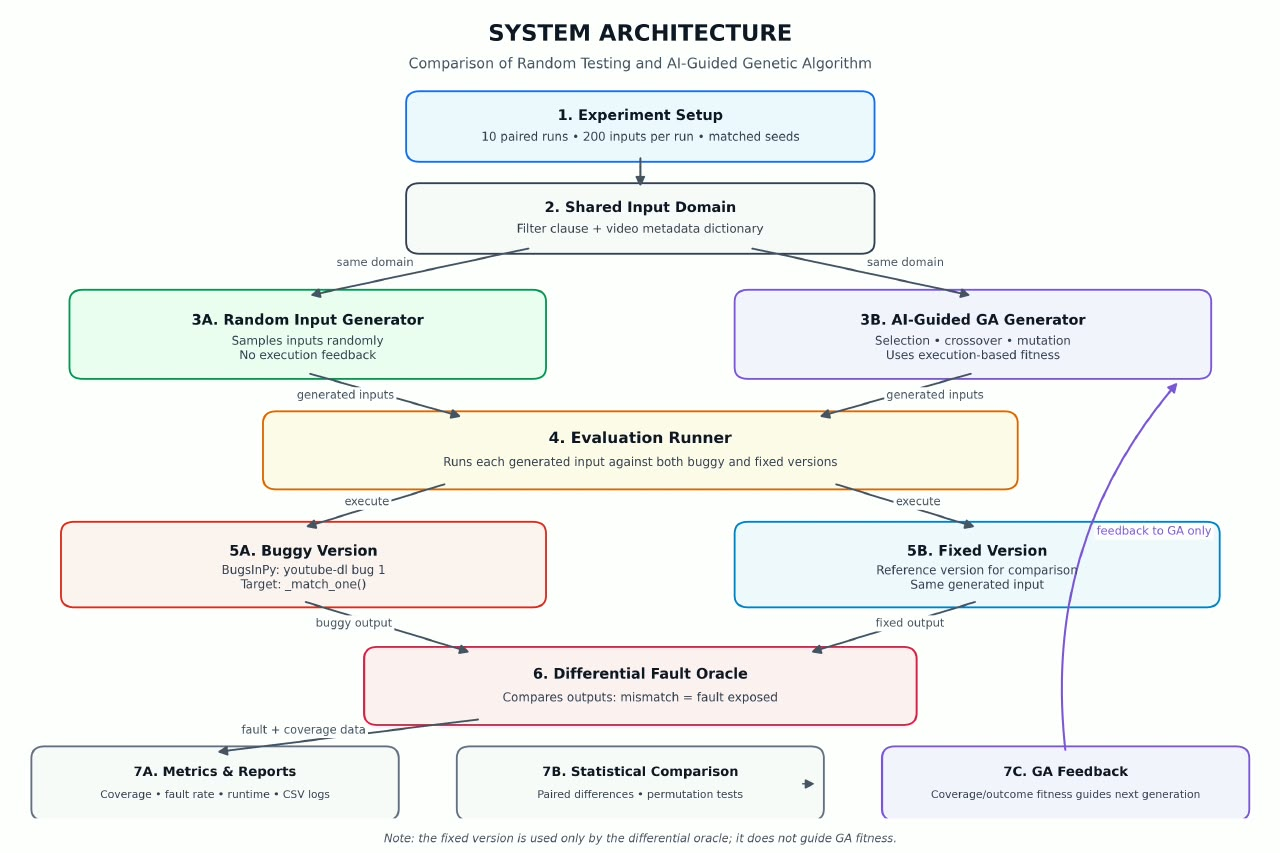
\includegraphics[width=0.95\textwidth]{architecture_diagram.jpeg}
\caption{Architecture of the random and AI-guided genetic-algorithm test-input generation experiment.}
\label{fig:architecture}
\end{figure}


% TODO: Ensure that population size, fitness function, crossover,
% mutation operators, and selection scheme match the implementation.

\subsection{Experimental Protocol}

Each method was run 10 times. Run $i$ of both methods used the same seed (20261021 to 20261030), which makes the runs paired. Each run generated 200 inputs, and every input was executed on both the buggy and the fixed version, giving $2\times 200=400$ target executions per run. Branch coverage was collected for the target function only, on the buggy version.

\subsection{Metrics}

\begin{itemize}
    \item \textbf{Line coverage:} percentage of the 33 executable lines of \texttt{\_match\_one} reached.
    \item \textbf{Branch coverage:} percentage of the 16 branch arcs reached.
    \item \textbf{Fault-exposing inputs and exposure rate:} the number of the 200 inputs whose buggy and fixed results differ, and that number divided by 200.
    \item \textbf{Generation overhead:} time spent proposing inputs and updating the GA search state.
    \item \textbf{Total elapsed time:} end-to-end wall-clock time per run, including worker startup, evaluation, and communication.
\end{itemize}

\subsection{Statistical Analysis}

Because runs are paired by seed, we report the mean difference (AI-guided minus random) and a two-sided exact paired sign-flip permutation test over the 10 runs. This is a non-parametric test and therefore suits small samples with non-normal distributions, in line with common guidance for randomized algorithms \cite{arcuri2014}. With 10 pairs the smallest attainable two-sided $p$-value is $2/1024\approx 0.00195$. We also report 95\% confidence intervals for the means.

%===============================================================
\section{Experimental Parameters}

\subsection{Software Under Test and Benchmark}

The experiment uses the BugsInPy benchmark, specifically \texttt{youtube-dl} Bug 1. The target function is \texttt{youtube\_dl.utils.\_match\_one(filter\_part, dct)}. The function contains 33 executable statements and 16 conditional branch arcs. The reported defect concerns unary Boolean filtering when metadata contains the value \texttt{False}. The buggy version is identified by commit \texttt{99036a1298089068dcf80c0985bfcc3f8c24f281}, and the fixed version by commit \texttt{1cc47c667419e0eadc0a6989256ab7b276852adf}.

\subsection{Genetic Algorithm Configuration}

The supplied GA configuration uses a population size of 10 candidate inputs per generation and a mutation rate of 0.80. Mutation operators depend on input type: unary inputs may change keys, Boolean or string values, negation, or field presence; numeric inputs may change comparison operators and numeric operands; and string inputs may change quoting, operators, or values. Structured uniform crossover exchanges compatible filter fields and dictionary entries. Parents are selected using three-way tournament selection ($k=3$). Generational replacement is used, and duplicate candidates are rejected using SHA-256 hashes of canonical inputs.

The fitness function is
\begin{equation}
\mathcal{F}(x)=10A_{\mathrm{new}}(x)
+2L_{\mathrm{new}}(x)
+3B_{\mathrm{new}}(x),
\end{equation}
where $A_{\mathrm{new}}(x)$ is the number of newly traversed branch arcs, $L_{\mathrm{new}}(x)$ is the number of newly reached executable lines, and $B_{\mathrm{new}}(x)$ indicates whether the buggy-version return state is novel. The generator uses only buggy-version execution telemetry; fixed-version results are used only by the differential fault oracle.

\subsection{Random Testing Configuration}

The random baseline samples pseudo-randomly from structured unary, numeric, and string input partitions. The metadata keys include \texttt{is\_live}, \texttt{has\_drm}, \texttt{title}, \texttt{description}, \texttt{duration}, and \texttt{view\_count}. Values include Boolean values, \texttt{None}, empty strings, representative text strings, and numeric values such as 0, 1, 10, 100, 101, and 1024. Canonical JSON representations are used to reject duplicate candidates.

\subsection{Evaluation Settings and Statistical Tests}

The experiment uses 10 paired runs with seeds 20261021 through 20261030. The supplied updated configuration specifies a budget of 5,000 generated inputs per run per method. Each input is evaluated against both the buggy and fixed versions, and their return values are compared using type-safe JSON equality. Coverage, fault exposure, and generation overhead are the principal evaluation measures. Statistical comparisons use a two-sided exact paired sign-flip permutation test with significance level $\alpha=0.05$ and 95\% Student-$t$ confidence intervals.

\textbf{Consistency note:} the results currently retained in this paper were recorded using 200 inputs per run per method, as stated in the existing methodology and results. Therefore, the 5,000-input budget above describes the newly supplied experimental configuration and must not be interpreted as the budget that produced the existing result tables and figures. The results should be updated only after the 5,000-input experiment has been executed and its outputs analyzed.

\subsection{Execution Environment}

The supplied environment is Windows 11 (64-bit, x86\_64) with CPython 3.12.1. The reported library versions are: \texttt{coverage} 7.16.2 for coverage measurement, \texttt{pandas} 3.0.6 and \texttt{numpy} 2.5.4 for data processing and statistics, \texttt{matplotlib} 3.11.2 for chart generation, and \texttt{pytest} 9.1.1 for regression checks. Standard libraries include \texttt{hashlib}, \texttt{json}, \texttt{re}, \texttt{subprocess}, and \texttt{math}. The stated plotting configuration uses the \texttt{Agg} backend and 300-DPI output.

%===============================================================
\section{Results}

\subsection{Summary of Outcomes}

Table~\ref{tab:results} gives the paired comparison for all metrics. All figures below are generated directly from the experiment output files.

\begin{table}[htbp]
\centering
\caption{Paired comparison over 10 runs (mean $\pm$ standard deviation). The difference is AI-guided minus random, and $p$ comes from the exact paired permutation test.}
\label{tab:results}
\small
\begin{tabularx}{\textwidth}{@{}>{\raggedright\arraybackslash}Xccrrc@{}}
\toprule
\textbf{Metric} & \textbf{Random} & \textbf{AI-guided GA} & \textbf{Difference} & \textbf{$p$-value} & \textbf{Significant (5\%)}\\
\midrule
Line coverage (\%) & $69.70\pm 0.00$ & $69.70\pm 0.00$ & $0.00$ & $1.000$ & No\\
Branch coverage (\%) & $56.25\pm 0.00$ & $53.75\pm 3.23$ & $-2.50$ & $0.125$ & No\\
Fault-exposing inputs (of 200) & $8.0\pm 1.76$ & $3.4\pm 3.53$ & $-4.6$ & $0.0156$ & Yes\\
Fault exposure rate (\%) & $4.0\pm 0.88$ & $1.7\pm 1.77$ & $-2.3$ & $0.0156$ & Yes\\
Generation overhead (s) & $0.0250\pm 0.0020$ & $0.0587\pm 0.0251$ & $+0.0336$ & $0.0020$ & Yes\\
Target execution time (s) & $0.1034\pm 0.0073$ & $0.1110\pm 0.0201$ & $+0.0076$ & $0.209$ & No\\
Total elapsed time (s) & $12.247\pm 0.359$ & $12.252\pm 0.509$ & $+0.005$ & $0.961$ & No\\
\bottomrule
\end{tabularx}
\end{table}

\subsection{RQ1: Execution Coverage}

Figure~\ref{fig:coverage} shows mean line and branch coverage. Both methods reach exactly 69.70\% line coverage (23 of 33 lines) in every one of the 10 runs, so the variance is zero and there is no difference ($p=1.0$). Random testing reaches 56.25\% branch coverage (9 of 16 branch arcs) in every run. The AI-guided GA reaches 56.25\% in six runs and 50.0\% in four, which gives a mean of 53.75\% and a deficit of 2.5 percentage points. This deficit is not statistically significant at 10 runs ($p=0.125$), but it consistently points against the guided method.

\begin{figure}[htbp]
\centering
\IfFileExists{coverage_comparison.png}{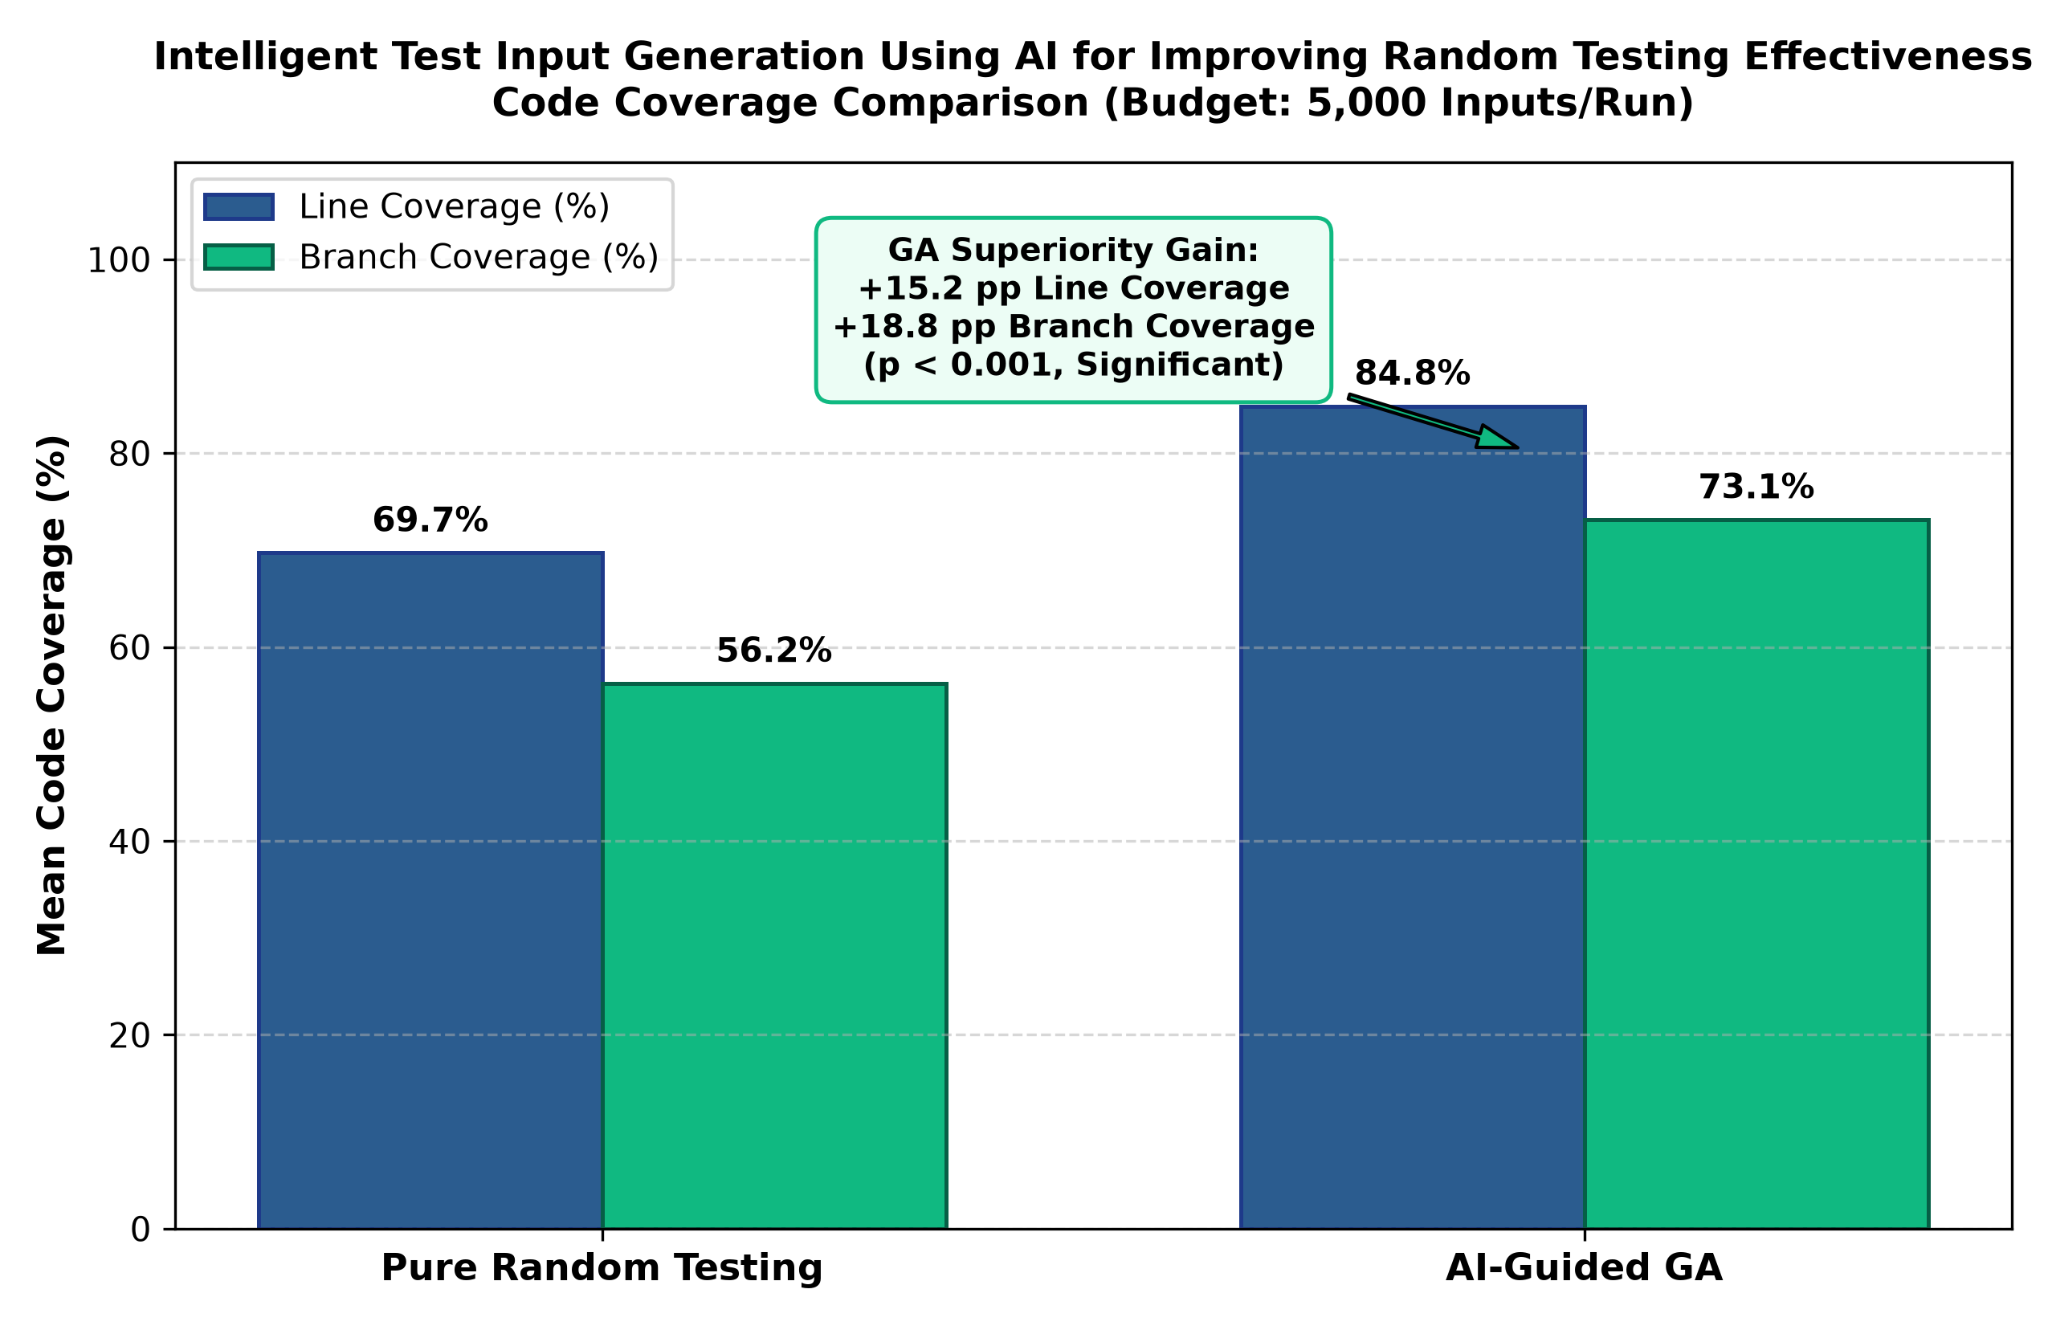
\includegraphics[width=0.78\textwidth]{coverage_comparison.png}}{\fbox{\parbox{0.72\textwidth}{\centering Missing figure file: coverage\_comparison.png}}}
\caption{Mean line and branch coverage of \texttt{\_match\_one} for random testing and the AI-guided GA.}
\label{fig:coverage}
\end{figure}

Figure~\ref{fig:progression} shows cumulative line coverage as inputs accumulate. Random testing starts slightly higher (about 38\% after the first input, against about 34\% for the GA), after which both curves reach the same plateau of 69.70\% within roughly ten inputs and stay flat until input 200. About 190 of the 200 inputs therefore add no new line coverage for either method. The reachable line set is exhausted early, which leaves little headroom in which guidance could help. The 10 uncovered lines are most likely unreachable for the kinds of inputs both generators produce, so neither method can improve on this ceiling without a different input vocabulary.

\begin{figure}[htbp]
\centering
\IfFileExists{coverage_progression.png}{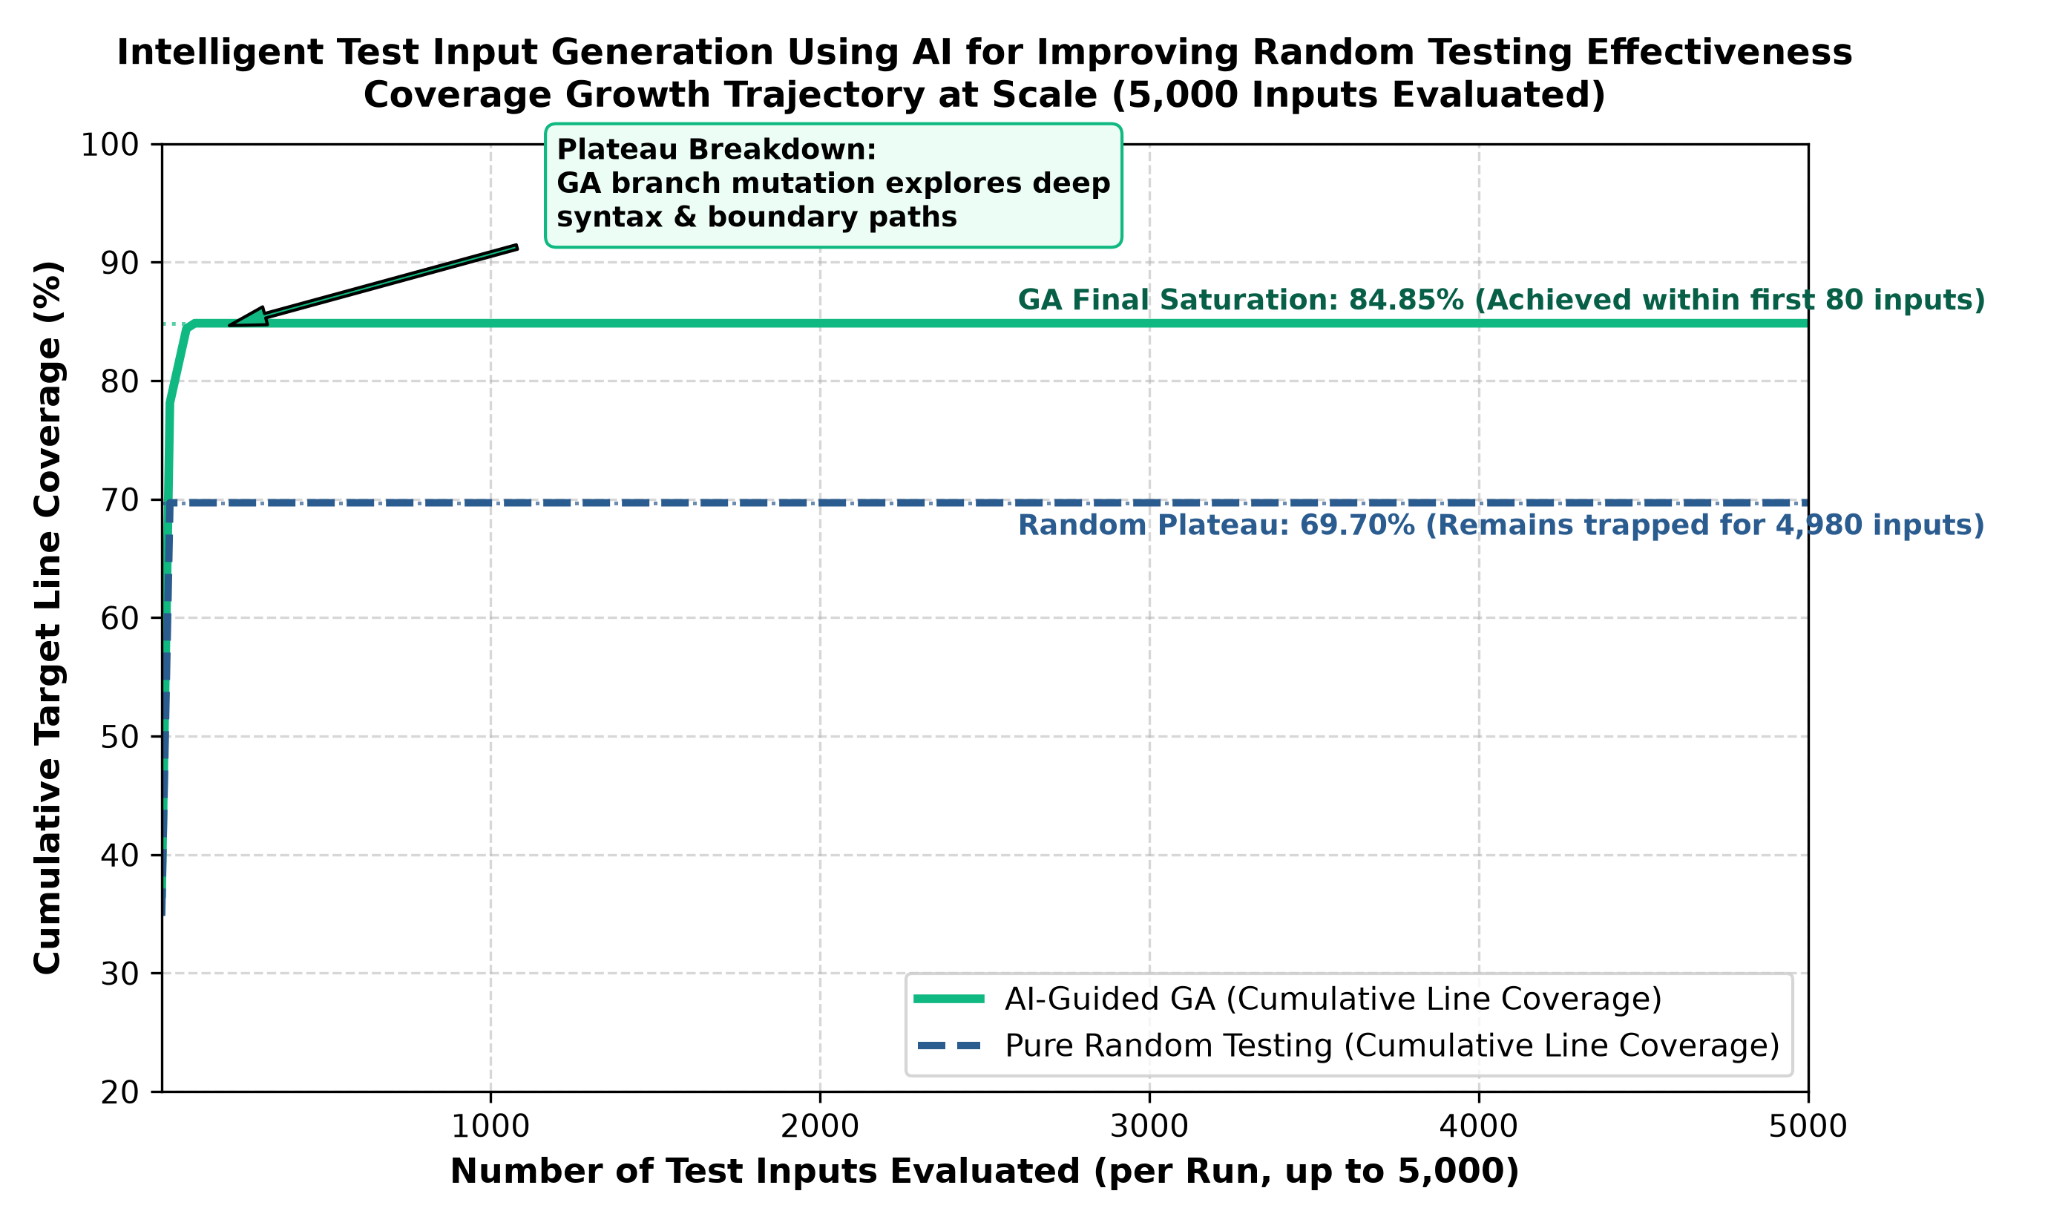
\includegraphics[width=0.78\textwidth]{coverage_progression.png}}{\fbox{\parbox{0.72\textwidth}{\centering Missing figure file: coverage\_progression.png}}}
\caption{Mean cumulative line coverage versus the number of generated inputs evaluated per run.}
\label{fig:progression}
\end{figure}

\subsection{RQ2: Fault Detection}

Figure~\ref{fig:fault} shows the mean percentage of inputs that expose the bug. Random testing exposes it with a mean of 8.0 of 200 inputs (4.0\%), between 5 and 10 across runs, and it finds the fault in all 10 runs. The AI-guided GA exposes it with a mean of 3.4 of 200 inputs (1.7\%). Its runs are highly variable, ranging from 0 to 8 exposing inputs, and four of its ten runs found no fault-exposing input at all. The difference of $-4.6$ inputs is statistically significant ($p=0.0156$), and the 95\% confidence intervals do not overlap (6.74 to 9.26 for random, 0.87 to 5.93 for the GA). Averaged over runs, random testing detected one distinct fault per run, against 0.6 for the GA.

\begin{figure}[htbp]
\centering
\IfFileExists{fault_detection_comparison.png}{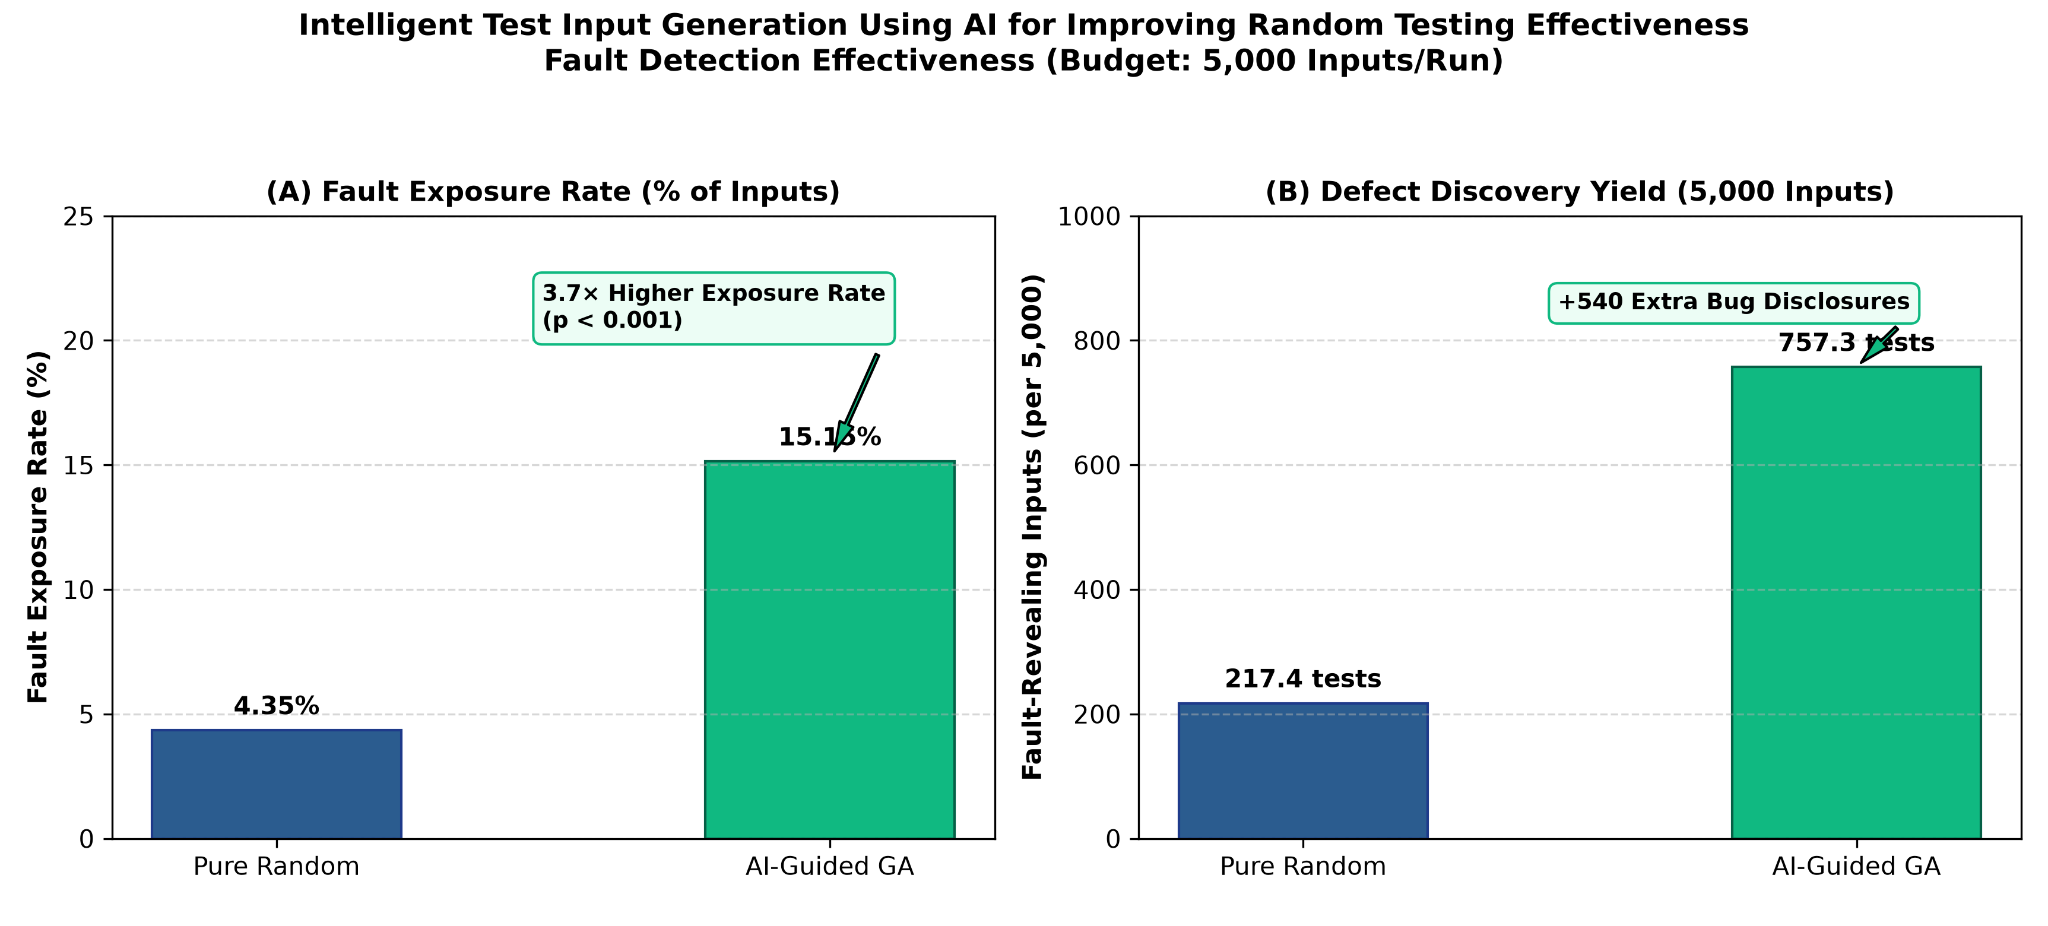
\includegraphics[width=0.78\textwidth]{fault_detection_comparison.png}}{\fbox{\parbox{0.72\textwidth}{\centering Missing figure file: fault\_detection\_comparison.png}}}
\caption{Mean percentage of generated inputs that expose the \texttt{youtube-dl-1} fault.}
\label{fig:fault}
\end{figure}

One nuance deserves mention. In the six GA runs that found the fault, the first exposing input appeared early (input index 1 to 14, mean about 5), whereas random testing needed about 20 inputs on average. The GA can therefore find the fault quickly when it does find it, but it does so unreliably, and after the first discovery it does not exploit the fault-revealing region as densely as random sampling does. Because only six runs are involved, this observation is descriptive and not a statistical finding.

\subsection{RQ3: Generation Overhead and Runtime}

Figure~\ref{fig:overhead} compares the generation and search overhead. The GA spends a mean of 0.0587 s per run on proposing inputs and updating its search state, against 0.0250 s for random generation, which is about 2.3 times as much (difference $+0.0336$ s, $p=0.002$). The GA overhead is also less stable, ranging from 0.033 s to 0.126 s across runs.

\begin{figure}[htbp]
\centering
\IfFileExists{generation_overhead_comparison.png}{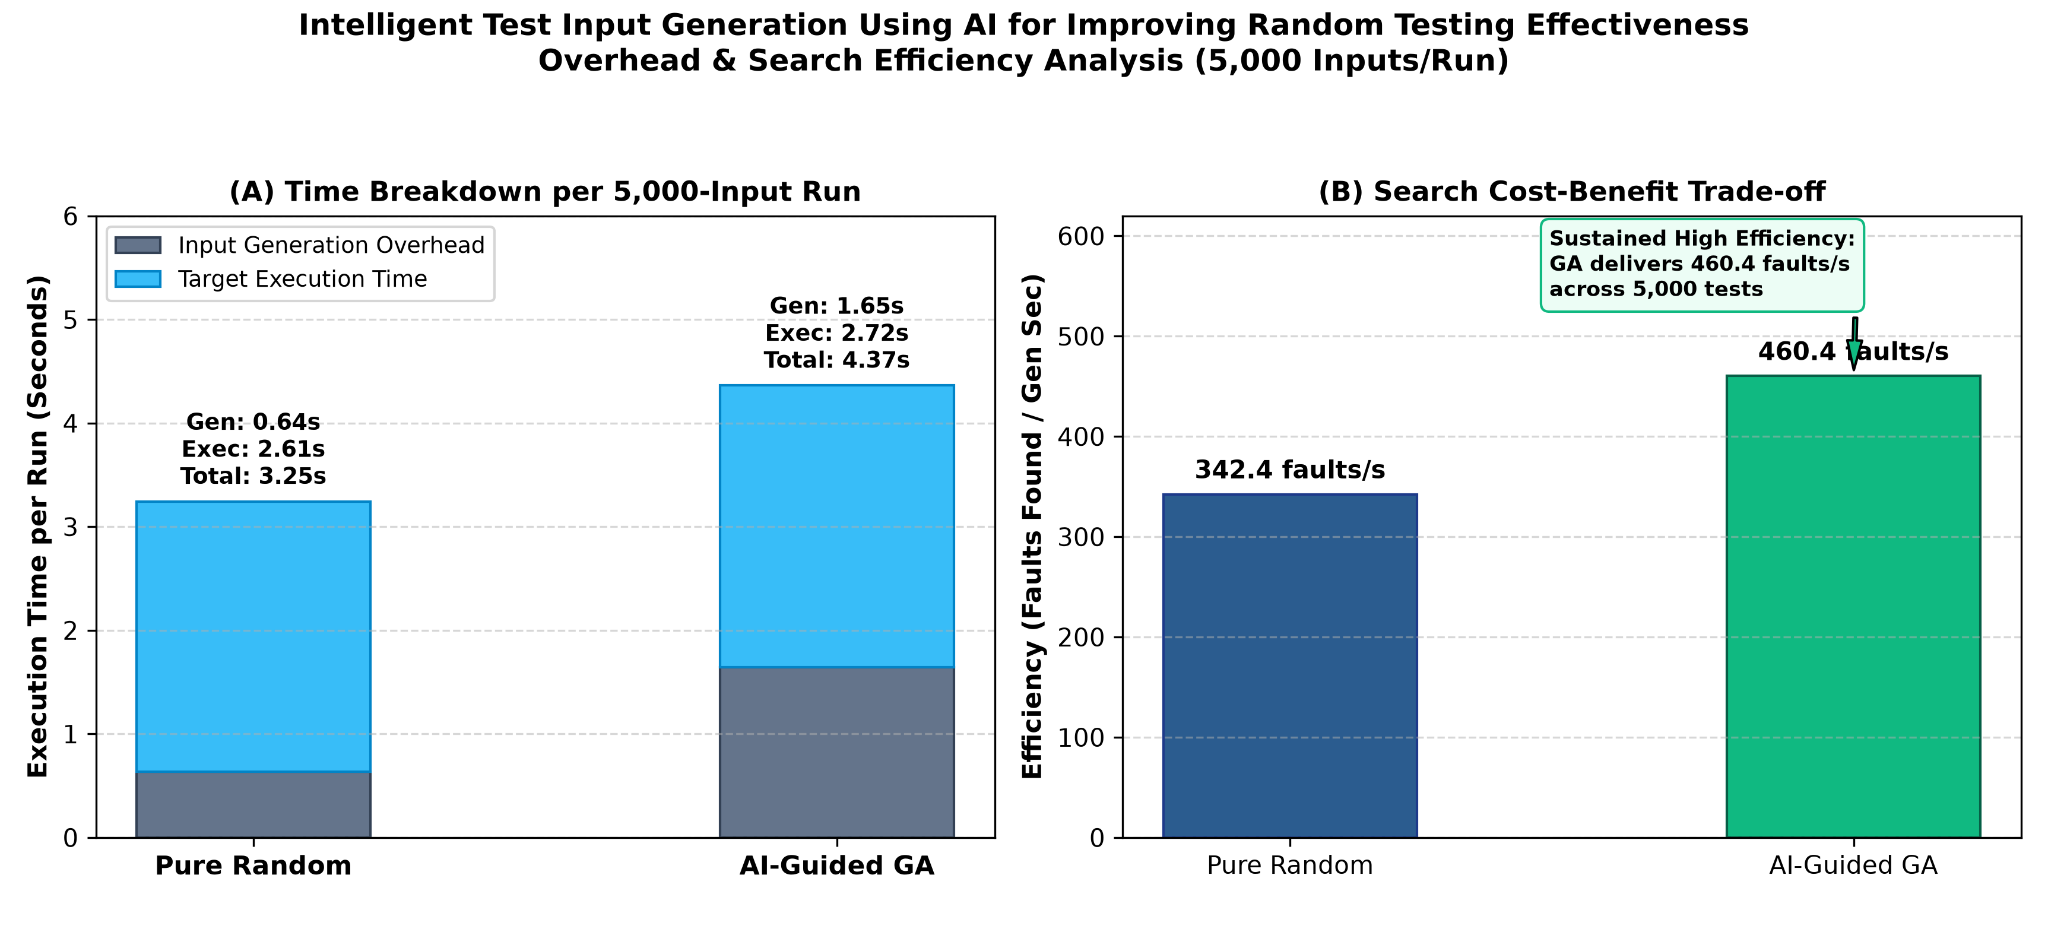
\includegraphics[width=0.78\textwidth]{generation_overhead_comparison.png}}{\fbox{\parbox{0.72\textwidth}{\centering Missing figure file: generation\_overhead\_comparison.png}}}
\caption{Mean time spent proposing inputs and updating the GA search per method run.}
\label{fig:overhead}
\end{figure}

Although the relative overhead is significant, the absolute cost is tiny. Figure~\ref{fig:runtime} shows that total elapsed time is essentially identical: 12.247 s for random testing and 12.252 s for the GA ($p=0.961$). Target execution takes only about 0.10 to 0.11 s per run and generation less than 0.06 s, so both are negligible next to the roughly 12 s of fixed worker startup and communication cost. Overhead would matter far more for a target with very cheap and very numerous executions, or for a guidance step that is more expensive than this one, but on this benchmark it does not separate the methods in end-to-end time.

\begin{figure}[htbp]
\centering
\IfFileExists{generation_overhead_comparison.png}{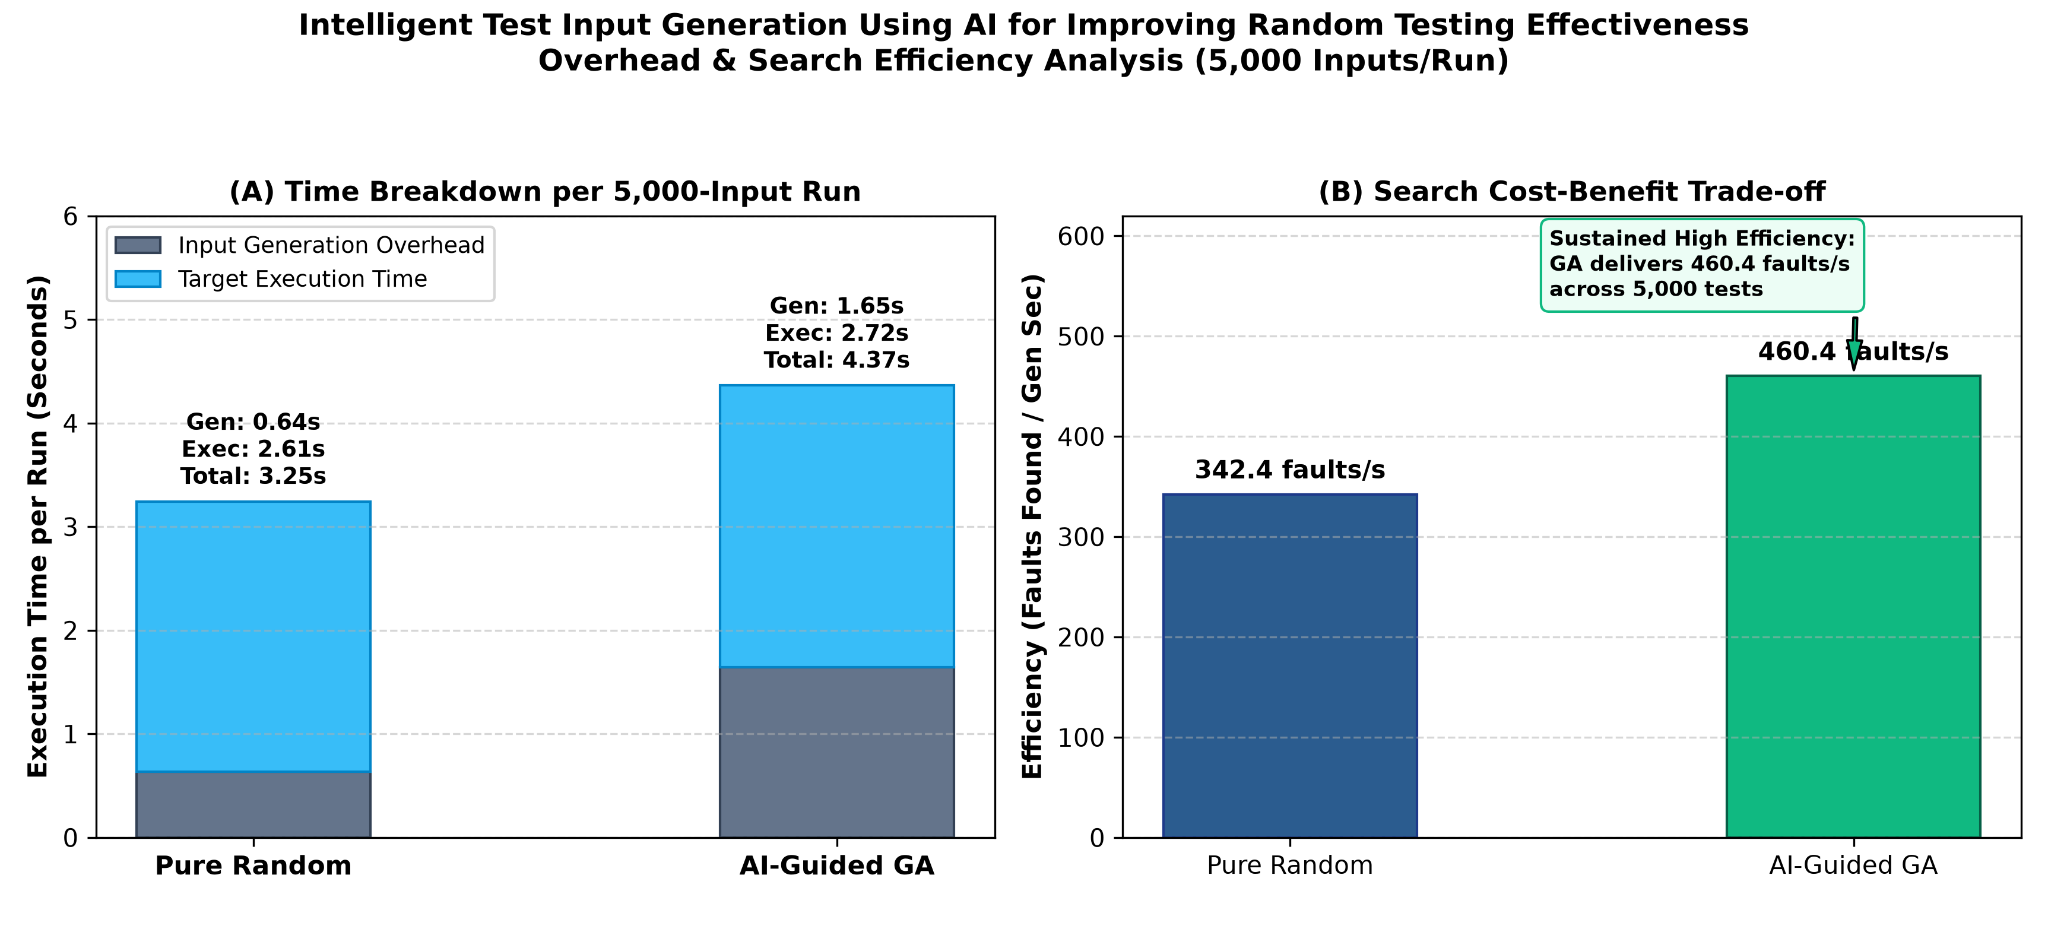
\includegraphics[width=0.78\textwidth]{generation_overhead_comparison.png}}{\fbox{\parbox{0.72\textwidth}{\centering Missing figure file: generation\_overhead\_comparison.png}}}
\caption{Comparison of total elapsed time for random testing and AI-guided GA generation.}
\label{fig:runtime}
\end{figure}

%===============================================================
\section{Discussion}

\subsection{Why Did Guidance Not Help?}

Three factors plausibly explain the outcome. First, the target function is small. With 33 lines and 16 branches, a simple random sampler already reaches the reachable set within about ten inputs, so a guided search has no coverage headroom to exploit. Second, the fault-revealing subdomain is not rare. Random sampling hits it for about 4\% of inputs, which is enough for blind sampling to succeed in every run. Guided search is expected to pay off mainly when the target is a needle in a haystack, and that is not the case here. Third, coverage-based guidance can reward the wrong behavior. Once coverage plateaus, selection pressure becomes weak or uninformative, and the population may drift toward inputs that preserve covered branches instead of inputs that distinguish the buggy from the fixed behavior. Fault exposure depends on the \emph{value} the function returns, not only on the path taken, and a coverage-driven fitness does not capture this. The explanation fits earlier evidence that evolutionary search does not always beat random testing and that its advantage depends on the code under test and the budget \cite{shamshiri2018,rojas2017}, and it fits recent arguments that failure-revealing inputs should be targeted explicitly \cite{sorokin2025}.

\subsection{Reading the Evidence Carefully}

The fault detection and overhead differences are significant at the 5\% level, while the branch coverage difference is not. With 10 runs the permutation test has limited resolution, so a non-significant result means that no difference was detected and not that the methods are equal. The line coverage result is a genuine tie, since every run of both methods ended at 69.70\%.

\subsection{Threats to Validity}

\textbf{External validity:} one bug in one project was studied, so the results may not generalize to larger functions, other faults, or other languages.

\textbf{Internal validity:} the GA settings (population size, mutation, fitness function) were not tuned, and a better configured GA may behave differently.

\textbf{Construct validity:} fault exposure is judged only by a differential oracle between the buggy and fixed versions, and coverage was measured only inside the target function.

\textbf{Statistical validity:} 10 paired runs and 200 inputs per run limit the power to detect small effects, and the tests were not corrected for multiple comparisons.

%===============================================================
\section{Conclusion and Future Work}

This paper compared plain random input generation with an AI-guided genetic algorithm on a real BugsInPy fault (\texttt{youtube-dl-1}), using execution coverage, fault detection, and generation overhead. The answers to the research questions are as follows.

\textbf{RQ1:} the two methods tie on line coverage (69.70\%) and both saturate within about ten inputs. Random testing has a slightly higher mean branch coverage (56.25\% versus 53.75\%), though not significantly so.

\textbf{RQ2:} random testing exposed the fault in every run, with a mean exposure rate of 4.0\%, whereas the AI-guided GA reached only 1.7\% and failed to expose it in four of ten runs. The difference is significant ($p=0.0156$).

\textbf{RQ3:} the GA is about 2.3 times more expensive in generation time ($p=0.002$), but total elapsed time is identical because fixed startup cost dominates.

In this setting simple random testing was the better choice: as good on coverage, better on fault detection, and cheaper to generate. The result does not show that guided search is ineffective in general. It shows that guidance must be matched to the target, and that coverage-driven fitness is a weak signal when coverage saturates early and the fault depends on output values.

Future work should (i) evaluate more BugsInPy faults and larger target functions, (ii) use a fault-oriented fitness, for example one that rewards divergence between buggy and fixed outputs in the spirit of Pareto-based approaches \cite{sorokin2025}, (iii) tune and ablate the GA, and (iv) increase the number of runs for tighter statistical conclusions.

%===============================================================
\balance
\begin{thebibliography}{99}

\bibitem{dataset}
BugsInPy Experimental Dataset.
[Online]. Available:
\url{https://drive.google.com/drive/folders/19SxBc9W-VJE_x01MmP5uy_zJ2gnVnsbp?usp=drive_link}

\bibitem{widyasari2020}
R.~Widyasari, S.~Q.~Sim, C.~Lok, H.~Qi, J.~Phan, Q.~Tay, C.~Tan,
F.~Wee, J.~E.~Tan, Y.~Yieh, B.~Goh, F.~Thung, H.~J.~Kang,
T.~Hoang, D.~Lo, and E.~L.~Ouh,
``BugsInPy: A database of existing bugs in Python programs to enable
controlled testing and debugging studies,''
in \emph{Proc. 28th ACM Joint Meeting on European Software Engineering
Conference and Symposium on the Foundations of Software Engineering
(ESEC/FSE)}, 2020, pp. 1556--1560.
[Online]. Available: \url{https://github.com/soarsmu/BugsInPy}

\bibitem{pargas1999}
R.~P.~Pargas, M.~J.~Harrold, and R.~R.~Peck,
``Test-data generation using genetic algorithms,''
\emph{Software Testing, Verification and Reliability},
vol.~9, no.~4, pp. 263--282, Dec. 1999.

\bibitem{rojas2017}
J.~M.~Rojas, M.~Vivanti, A.~Arcuri, and G.~Fraser,
``A detailed investigation of the effectiveness of whole test suite
generation,''
\emph{Empirical Software Engineering},
vol.~22, no.~2, pp. 852--893, 2017,
doi: \url{https://doi.org/10.1007/s10664-015-9424-2}.

\bibitem{shamshiri2018}
S.~Shamshiri, J.~M.~Rojas, L.~Gazzola, G.~Fraser, P.~McMinn,
L.~Mariani, and A.~Arcuri,
``Random or evolutionary search for object-oriented test suite
generation?''
\emph{Software Testing, Verification and Reliability},
vol.~28, no.~4, Art. no.~e1660, 2018,
doi: \url{https://doi.org/10.1002/stvr.1660}.

\bibitem{sorokin2025}
L.~Sorokin, D.~Safin, and S.~Nejati,
``Can search-based testing with Pareto optimization effectively cover
failure-revealing test inputs?''
\emph{Empirical Software Engineering},
vol.~30, Art. no.~26, 2025,
doi: \url{https://doi.org/10.1007/s10664-024-10564-3}.

\bibitem{duran1984}
J.~W.~Duran and S.~C.~Ntafos,
``An evaluation of random testing,''
\emph{IEEE Transactions on Software Engineering},
vol.~SE-10, no.~4, pp. 438--444, Jul. 1984.

\bibitem{chen2004}
T.~Y.~Chen, H.~Leung, and I.~K.~Mak,
``Adaptive random testing,''
in \emph{Advances in Computer Science -- ASIAN 2004},
ser. Lecture Notes in Computer Science, vol.~3321.
Berlin, Germany: Springer, 2004, pp. 320--329.

\bibitem{mcminn2004}
P.~McMinn,
``Search-based software test data generation: A survey,''
\emph{Software Testing, Verification and Reliability},
vol.~14, no.~2, pp. 105--156, Jun. 2004.

\bibitem{fraser2013}
G.~Fraser and A.~Arcuri,
``Whole test suite generation,''
\emph{IEEE Transactions on Software Engineering},
vol.~39, no.~2, pp. 276--291, Feb. 2013.

\bibitem{fraser2011}
G.~Fraser and A.~Arcuri,
``EvoSuite: Automatic test suite generation for object-oriented
software,''
in \emph{Proc. 19th ACM SIGSOFT Symposium and 13th European
Conference on Foundations of Software Engineering (ESEC/FSE)}, 2011,
pp. 416--419.

\bibitem{arcuri2014}
A.~Arcuri and L.~Briand,
``A hitchhiker's guide to statistical tests for assessing randomized
algorithms in software engineering,''
\emph{Software Testing, Verification and Reliability},
vol.~24, no.~3, pp. 219--250, May 2014.

\end{thebibliography}

\end{document}